%% Follow comments to support use.

%%%%%%%%%%%%%%%%%%%%%%%%%%%%%%%%%%%%%%%%%%%%%%%%%%%%%%%%%
%% STEP 1: Choose options for MSc / BSc / seminar layout and your bibliographic style
%%%%%%%%%%%%%%%%%%%%%%%%%%%%%%%%%%%%%%%%%%%%%%%%%%%%%%%%%

%%  Language:
%%      finnish, swedish, or english
%%  Pagination (use twoside by default)
%%      oneside or twoside,
%%  Study programme / kind of report
%%      csm  = Master's thesis in Computer Science Master's Programme;
%%      tkt = Bachelor's thesis in Computer Science Bachelor's Programme;
%%      seminar = seminar report
%%  For Master's thesis choose your line or track:
%%      (30 cr thesis, 2020 onwards, Master's Programme in Computer Science = csm)
%%      software-track-2020 = Software study track
%%      algorithms-track-2020 = Algorithms study track
%%      networking-track-2020 = Networking study track

\documentclass[english,twoside,censored,tkt]{HYthesisML}

\newif\ifcomments
\commentstrue
%\commentsfalse

\newcommand{\citetemp}{
\ifcomments
    \textcolor{red}{[!]}
\fi
}
\newcommand{\comment }[1]{
   \ifcomments
    \emph{\textcolor{blue}{ (#1) }}
   \fi
}
% If wanted, open new chapters only at right page.
% By default, "openany".
%\PassOptionsToClass{openright,twoside,a4paper}{report}
\PassOptionsToClass{openany,twoside,a4paper}{report}

\usepackage{csquotes}
%%%%%%%%%%%%%%%%%%%%%%%%%%%%%%%%%%%%%%%%%%%%%%%%%%%%%%%%%
%% REFERENCES
%% Some notes on bibliography usage and options:
%% natbib -> you can use, e.g., \citep{} or \parencite{} for (Einstein, 1905); with APA \cite -> Einstein, 1905 without ()
%% maxcitenames=2 -> only 2 author names in text citations, if more -> et al. is used
%% maxbibnames=99 as no great need to suppress the biliography list in a thesis
%% for more information see biblatex package documentation, e.g., from https://ctan.org/pkg/biblatex

%% Reference style: select one
%% for APA = Harvard style = authoryear -> (Einstein, 1905) use:
% \usepackage[style=authoryear,bibstyle=authoryear,backend=biber,natbib=true,maxnames=99,maxcitenames=2,uniquelist=minyear,giveninits=true,uniquename=mininit]{biblatex}
%% for numeric = Vancouver style -> [1] use:
\usepackage[style=numeric,bibstyle=numeric,backend=biber,natbib=true,maxbibnames=99,giveninits=true,uniquename=init]{biblatex}
%% for alpahbetic -> [Ein05] use:
%\usepackage[style=alphabetic,bibstyle=alphabetic,backend=biber,natbib=true,maxbibnames=99,giveninits=true,uniquename=init]{biblatex}
%

\addbibresource{bibliography.bib}
% in case you want the final delimiter between authors & -> (Einstein & Zweistein, 1905)
% \renewcommand{\finalnamedelim}{ \& }
% List the authors in the Bibilipgraphy as Lastname F, Familyname G,
\DeclareNameAlias{sortname}{family-given}
% remove the punctuation between author names in Bibliography
%\renewcommand{\revsdnamepunct}{ }

% Asked chat.openai.com: I'm using biblatex package, but it prints odd format volume.number in reference list, while this should be volume (number). How to fix this?
%Answer (shortened):
% Redefine the volume and number format
%\DeclareFieldFormat[article]{volume}{\mkbibbold{#1}}
%\DeclareFieldFormat[article]{number}{\mkbibparens{#1}}
% Please remove the boldface from the volume and number fields:
\DeclareFieldFormat[article]{volume}{#1}
\DeclareFieldFormat[article]{number}{\mkbibparens{#1}}
% Now this generated format volume.(number). How to remove the dot? (and so on with some adjustments):
\renewbibmacro*{volume+number+eid}{%
  \setunit{\addcomma\space}%
  \printfield{volume}%
  %\setunit*{\addnbspace\addthinspace}% <-- Adjust spacing here
  \printfield{number}%
  \setunit{\addcomma\space}%
  \printfield{eid}}


%% Block of definitions for fonts and packages for picture management.
%% In some systems, the figure packages may not be happy together.
%% Choose the ones you need.

%\usepackage[utf8]{inputenc} % For UTF8 support, in some systems. Use UTF8 when saving your file.

\usepackage{lmodern}         % Font package, again in some systems.
\usepackage{textcomp}        % Package for special symbols
\usepackage[pdftex]{color, graphicx} % For pdf output and jpg/png graphics
\usepackage{epsfig}
\usepackage[pdftex, plainpages=false]{hyperref} % For hyperlinks and pdf metadata
\usepackage{fancyhdr}        % For nicer page headers
\usepackage{tikz}            % For making vector graphics (hard to learn but powerful)
%\usepackage{wrapfig}        % For nice text-wrapping figures (use at own discretion)
\usepackage{amsmath, amssymb} % For better math
\usepackage{pgfplots}
\usepackage{array, booktabs}
\usepackage{listings}
\usepackage{xcolor}


% Define styles for lstlisting
\lstset{
  language=Python,
  basicstyle=\ttfamily\small,
  keywordstyle=\color{blue}\bfseries,
  commentstyle=\color{gray},
  stringstyle=\color{teal},
  showstringspaces=false,
  frame=single,
  numbers=left,
  numberstyle=\tiny\color{gray},
  breaklines=true,
  captionpos=b,
  xleftmargin=2em,
  framexleftmargin=1.5em,
}
\pgfplotsset{compat=1.18}
\singlespacing               %line spacing options; normally use single

\fussy
%\sloppy                      % sloppy and fussy commands can be used to avoid overlong text lines
% if you want to see which lines are too long or have too little stuff, comment out the following lines
% \overfullrule=1mm
% to see more info in the detailed log about under/overfull boxes...
% \showboxbreadth=50
% \showboxd epth=50



%%%%%%%%%%%%%%%%%%%%%%%%%%%%%%%%%%%%%%%%%%%%%%%%%%%%%%%%%
%% STEP 2:
%%%%%%%%%%%%%%%%%%%%%%%%%%%%%%%%%%%%%%%%%%%%%%%%%%%%%%%%%
%% Set up personal information for the title page and the abstract form.
%% Replace parameters with your information.
\title{Python Type Annotations: Adoption and Benefits}

\author{Kerkko Pelttari}
\date{\today}

% Set supervisors, use the titles according to the thesis language
% in English Prof. or Dr., or in Finnish toht. or tri or FT, TkT, Ph.D. or in Swedish...
\supervisors{Prof. Dorota Glowacka, Dr. Yang Liu}

\keywords{Python, Type systems, Type annotations, Type checking, Gradual typing}
\additionalinformation{\translate{\track}}

%% For seminar reports:
%%\additionalinformation{Name of the seminar}

%% Provide classification terms, to appear on the abstract page.
%% Replace the classification terms below with the ones that match your work.
%% ACM Digital library provides a taxonomy and a tool for classification
%% in computer science. Use 1-3 paths, and use right arrows between the
%% about three levels in the path; each path requires a new line.

\classification{\protect{\ \\
\  Software and its engineering $\rightarrow$ Software notations and tools  $\rightarrow$ General programming languages\  \\
\ $\rightarrow$ Language features

\  Software and its engineering $\rightarrow$ Software creation and management
\  $\rightarrow$ Software development techniques
}}


% Finally, specify 1--3 ACM Computing Classification System (CCS) topics, as per \url{https://dl.acm.org/ccs}.
% Each topic is specified with one path, as shown in the example below, and elements of the path separated with an arrow.
% Emphasis of each element individually can be indicated
% by the use of bold face for high importance or italics for intermediate level.


%% If you want to quote someone special. You can comment this line out and there will be nothing on the document.
%\quoting{Bachelor's degrees make pretty good placemats if you get them laminated.}{Jeph Jacques}


%% OPTIONAL STEP: Set up properties and metadata for the pdf file that pdfLaTeX makes.
%% Your name, work title, and keywords are recommended.
\hypersetup{
    unicode=true,           % to show non-Latin characters in Acrobat’s bookmarks
    pdftoolbar=true,        % show Acrobat’s toolbar?
    pdfmenubar=true,        % show Acrobat’s menu?
    pdffitwindow=false,     % window fit to page when opened
    pdfstartview={FitH},    % fits the width of the page to the window
    pdftitle={Python Type Annotations: Usage and Benefits},            % title
    pdfauthor={Kerkko Pelttari},           % author
    pdfsubject={},          % subject of the document
    pdfcreator={},          % creator of the document
    pdfproducer={pdfLaTeX}, % producer of the document
    pdfkeywords={python} {type systems} {type annotations}, % list of keywords for
    pdfnewwindow=true,      % links in new window
    colorlinks=true,        % false: boxed links; true: colored links
    linkcolor=black,        % color of internal links
    citecolor=black,        % color of links to bibliography
    filecolor=magenta,      % color of file links
    urlcolor=cyan           % color of external links
}
\usepackage{caption}
\usepackage{subcaption} % replaces subfigure with better features
%%-----------------------------------------------------------------------------------

\begin{document}

% Generate title page.
\maketitle

%%%%%%%%%%%%%%%%%%%%%%%%%%%%%%%%%%%%%%%%%%%%%%%%%%%%%%%%%
%% STEP 3:
%%%%%%%%%%%%%%%%%%%%%%%%%%%%%%%%%%%%%%%%%%%%%%%%%%%%%%%%%
%% Write your abstract in the separate file, to be positioned here.
%% You can make several abstract pages (if you want it in different languages),
%% in which case you should also define the language of the abstract,
%% as below.

% \begin{abstract}{finnish}

% Tämä dokumentti on tarkoitettu Helsingin yliopiston tietojenkäsittelytieteen osaston opin\-näyt\-teiden ja harjoitustöiden ulkoasun ohjeeksi ja mallipohjaksi. Ohje soveltuu kanditutkielmiin, ohjelmistotuotantoprojekteihin, seminaareihin ja maisterintutkielmiin. Tämän ohjeen lisäksi on seurattava niitä ohjeita, jotka opastavat valitsemaan kuhunkin osioon tieteellisesti kiinnostavaa, syvällisesti pohdittua sisältöä.


% Työn aihe luokitellaan  
% ACM Computing Classification System (CCS) mukaisesti, 
% ks.\ \url{https://dl.acm.org/ccs}. 
% Käytä muutamaa termipolkua (1--3), jotka alkavat juuritermistä ja joissa polun tarkentuvat luokat erotetaan toisistaan oikealle osoittavalla nuolella.

% \end{abstract}

\begin{otherlanguage}{english}
\begin{abstract}

This thesis is a literature review on Python type annotations, their use and benefits. Background on Python, type systems, type annotations and type checking is provided. Then the relevant literature is discussed and analysed.

Python is a widely utilized general purpose programming language. It's type system is strong and dynamic. In 2015 support for optional type annotations was implemented.

Python is well-known as simple, concise and readable. Type annotations may sometimes come in conflict with these. However the gradual nature of optional typing enables developers to choose and pick where to utilize type annotations. Type annotations have had a significant rise in popularity from 2015 to 2022. Still only a minority of Python source code utilizes them. Python type inference and checking has been integrated into code editors, and this helps developers work with both typed and untyped source code.

Existing research has determined that it is possible to find approximately 15\% software defects (bugs) by utilizing type annotations. Type annotations can be utilized to document public interfaces and to ensure correctness in desired areas.

\comment{
Finally, specify 1--3 ACM Computing Classification System (CCS) topics, as per \url{https://dl.acm.org/ccs}.
Each topic is specified with one path, as shown in the example below, and elements of the path separated with an arrow.
Emphasis of each element individually can be indicated
by the use of bold face for high importance or italics for intermediate
level.}

\end{abstract}
\end{otherlanguage}

\begin{otherlanguage}{finnish}
\section*{Lyhennelmä}

TODOs:
    - wikipedia:
        - https://fi.wikipedia.org/wiki/Tyyppij%C3%A4rjestelm%C3%A4#Staattinen_vs._dynaaminen_tyypitys
            - Staattinen vs. dynaaminen tyypitys
            - Staattinen - dynaaminen tyypitys kahtiajako
            - TODO: tänne vois lisää vähittäisen tyypityksen
    - mahdollisesti leikkaa: (bugien)

Lista termikäännöksistä:
    - TODO: termeille joille ei ole kovin vakiintunutta suomennusta hyvä mainita enkkutermit tarkennuksina
    - gradual typing: Vähittäinen tyypitys
    - type hint: tyyppivihje
    - type annotation: ? (ihan vaan tyyppivihje?)
        - Tarvisko
    - type information: tyyppi-informaatio
        TODO: tarkista
    - unchecked exception: käsittelemätön poikkeus
    - superset (tyyppijärjestelmienkin kontekstissa): ylijoukko
    - whitespace: ??
        - symbolit välistys, merkitsevä indentaatio ja rivivaihdot
    - scripting: komentosarjaohjelmointi (scripting)
    - refactor: refaktorointi
    - onko "tyypitetty python" selkeä? Pitäiskö se esitellä terminä?
        esittely: (jatkossa tyypitetty Python)
    - "scrape a dataset" (joka oli kontekstissa vähän väärä termi): ottaa satunnaisotanta
    - bug: ohjelmointivirhe
    - codebase: ??
    - commit: muutos
    - null safety: ??

- Plan:

- Introduction

    - Python on laajasti käytetty ohjelmointikieli. Vuonna 2015 siihen lisättiin tuki valinnaisille tyyppivihjeille, jotka mahdollistavat uudenlaisen tyyppitiedon lisäämisen lähdekoodiin.
    - Pythonin kasvava suosio ja Pythonin tyypitysratkaisujen kasvava suosio nostavat esiin ristiriidan: Miksi käyttää dynaamisesti tyypitettyä kieltä ja tyypittää koodi staattisesti?
    - Staattisissa kielissä ohjelma tyypitetään kääntäessä. Dynaamisessa kielessä tyypit päätetään ajonaikaisesti. Valinta näiden välillä vaikuttaa siihen milloin tyyppivirheitä havaitaan, ja siirtää oikeellisuuden varmistamista käännös- ja ajonaikaisen välillä.
    - Staattisen tai dynaamisen ohjelmointikielen valinnalla vaikuttaa joskus olevan tilastollisesti havaittava vaikutus ohjelmakoodin oikeellisuuteen \cite{nanz_comparative_2015, ray_codequality_2014}. Kuitenkin tulos paljon viitatusta vuoden 2014 tutkimuksesta \cite{ray_codequality_2014} ei toistunut vuonna 2019 suoritetussa toistotutkimuksessa \cite{codequality_reproudction_2019}. Havaitaan että ohjelmointikielillä kirjoitettujen ohjelmien oikeellisuuden vertailu on vaikeaa, sillä ohjelmointikielillä on monenlaisia eroja jotka tekevät oikeellisuuserojen vaikutuksen eristämisestä haastavaa.
    - Python tyyppivihjeillä on vähittäisesti tyypitetty ohjelmointikieli (jatkossa tyypitetty Python). Sillä kirjoitetut ohjelmat omaavat sekä staattisen että dynaamisen kielen piirteitä. Vähittäisen tyypityksen ratkaisuista, kuten JavaScript ohjelmien tyypityksen laajentamisesta TypeScriptillä, voidaan hvaita tilastollisesti merkittäviä parannuksia ohjelmointivirheiden (bugien) havaitsemisessa. \cite{gao_to_type_or_not_2017}. Tyyppivihjeillä varustetulle Pythonille on löydetty lupaavia tuloksia bugien havainnoinnista tyypittämättömään Pythoniin verrattuna \cite{khan_empirical_2022, rak-amnouykit_taleoftwo_2020}
    - <lukukuvaukset>

- Background
    - Tyyppijärjestelmät
            TODO: alla olevan voisi muotoilla paremmin
        - Tyyppijärjestelmät antavat organisoida ja kategorisoida ohjelman tilaa, informaatiota, funktioita, ja näihin liittyviä rakenteita \cite{programming_langs}. Niiden avulla ohjelmointikieli voi antaa takeita ohjelman toiminnasta, valita miten dataa käsitellään, ja tyyppi-informaatio voi toimia tarkistettavavana lisäinformaationa ohjelman rakenteesta.

        - Käytännössä kaikki korkean tason ohjelmointikielet hyödyntävät tyyppijärjestelmää. Tyyppijärjestelmien ominaisuudet, hienojakoisuus, rajoitteet ja päättelylogiikka vaihtelevat. Ohjelmointikielet voidaan jakaa erinäisiin akseleihin: vahvasti ja heikosti tyypitettyihin, ja staattisesti, dynaamisesti tai vähittäin tyypitettyihin.

    - Vahvat ja heikot tyyppijärjestelmät
        - Vahvassa tyyppijärjestelmässä ei sallita käsittelemättömiä tyyppivirheitä \cite{cardelli_typeful_1989}. Tyyppivirheen tapahtuessa vahvasti tyypitetyn ohjelmointikielen on pakko antaa virhe ohjelmoijalle käsiteltäväksi, tai kaatua.
        - Heikosti tyypitetyssä ohjelmointikielessä tyyppivirheen tapahtuessa se voidaan nostaa käsiteltäväksi virheeksi, mutta yleensä suoritetaan jonkinlainen implisiittinen tyyppimuunnos. Tämä voi joskus olla käytännöllistä, mutta voi johtaa virheelliseen toimintaan jonka tarkka syy on vaikea löytää.
    - Staattinen tyypitys
        - Staattisesti tyypitetyssä ohjelmointikielessä jokaisella symbolille on löydyttävä tai voitava päätellä oikea tyyppi tyyppitarkistuksessa, joka yleensä suoritetaan ohjelmakoodin kääntämisen yhteydessä. Teoriassa staattisesti tyypitetylle kielelle voidaan tarjota kattavampia ohjelmointityökaluja, sillä työkaluilla on enemmän informaatiota käytettävissä.

    - Dynaaminen tyypitys
        - Dynaamisesti tyypitetyssä kielessä tyypit symboleille selviävät vasta suorituksen aikana. Tämä mahdollistaa kevyemmän syntaksin, jossa ohjelmoijan ei tarvitse käyttää aikaa tyyppimäärittelyihin \cite{di_grazia_evolution_2022}.


    - Vähittäinen tyypitys
        - Vähittäiset tyypitysjärjestelmät muodostavat ylijoukon sekä staattisista että dynaamisista ohjelmointikielistä \cite{siek_refined_gradual_2015}. Vähittäisesti tyypitetyllä kielellä voi kirjoittaa sekä täysin staattisia että täysin dynaamisia ohjelmia, ja näiden välimuotoja. Erityisenä hyötynä tämä mahdollistaa ohjelmien tyypittämisessä keskittyä hyödyllisimpiin osioihin, ja kehittää tyyppikattavuutta vähitellen \cite{siek_refined_gradual_2015}. Usein vähittäiset tyyppijärjestelmät toteutetuaan olemassaolevan ohjelmointikielen päälle, kuten Pythonissakin.
        TODO: whitespace
    - Python on korkean tason tulkattu ohjelmointikielen joka on tiivis ja ilmaisuvoimainen. Pythonin tyyppijärjestelmä on vahva ja dynaaminen. Sitä käytetään esimerkiksi tieteelliseen laskentaan, koneoppimiseen, verkkopalvelukehitykseen ja komentosarjaohjelmointiin (scripting).
    - Tyypit Pythonissa
        - Tyypitetyssä Pythonissa on kaksi tyyppijärjestelmää: 1) Ajonaikainen, dynaaminen, ohjelman toimintaa ohjaava järjestelmä. 2) Valinnainen tyyppivihjeisiin ja päättelyyn pohjaava järjestelmä joka lisättiin vuonna 2014 \cite{pep_484}. Nämä tyyppivihjeet eivät itsessään vaikuta ohjelman ajonaikaiseen käytökseen, mutta niitä hyödynnetään työkaluissa ja tarkistimissa.
    - Tyyppivihjeet
        - Keskitymme tarkastelemaan tyyppijärjestelmää 2). Tyyppivihjeiden tarkistamisen vapaaehtoisuus noudattaa \emph{vähittäistakuuta} (gradual guarantee), jonka mukaan saman ohjelman tyypitetyn ja tyypittämättömän version eroavaisuuksien tulisi rajoittua niiden tyyppeihin \cite{siek_refined_gradual_2015}. Pythonissa tyyppivihjeitä merkitään kaksoispisteellä muuttujille ja argumenteille {\tt x: int} ja nuolella funktioiden palautusarvoille {\tt def f() -> int: return 1}.
    - Tyyppitarkistus Pythonissa
        - Pythonille on kolme laajasti käytössä olevaa työkalua jotka tyyppitarkistavat: mypy, Pyright, ja PyCharm.
        TODO: sano jotain näistä?

    - Tyyppipäättely
        - Kaikki mainitut tyyppejä tarkistavat työkalut hyödyntävät tyyppipäättelyä \cite{jetbrains_type_hinting_pycharm, mypy_type_inference, pyright_type_inference}. Tyyppivihjeiden lisäksi ne pystyvät siis päättelemään muuttujien tyyppejä niihin asetettujen arvojen avulla, ja palautusarvoja palautettujen muuttujien tyyppien avulla. Tyyppipäättely mahdollistaa tyypityksen hyötyjä myös tyypittämättömään koodiin, koodin täydennykseen ja virheiden havainnointiin.

- Existing research
    - Yleisin metodi Python-tyyppiannotaatioiden oikeellisuuden tutkimiseen on ottaa satunnaisotanta Python ohjelmia ja ajaa tyyppitarkistuksia sitä vasten \cite{di_grazia_evolution_2022, lin_towards_large_scale_2023, rak-amnouykit_taleoftwo_2020, xu_how_well_static_2023}. Tämän avulla saadaan dataa tyyppikattavuudesta ja tyyppivirheistä. Kun halutaan tutkia miten hyvin tyyppitarkistimet löytävät korjattavaksi priorisoituja ohjelmointivirheitä, voidaan ottaa otanta korjatuista virheistä. Lisäämällä ohjelmointivirheen sisältävään ohjelmakoodiin tyyppivihjeet voidaan tyyppitarkistimella tarkistaa olisiko virhe näkynyt tyyppivirheiden muodossa.
    - % Usage practices
    - Funktioiden tyyppikattavuus on noussut 0\% lisäämisvuonna 2015 noin 8\% vuoteen 2021 mennessä, kuten näkyy kuvaajassa \ref{fig:annotation-evolution}. Toinen tuoreempi tutkimus selvitti tyyppikattavuutta yhdessä suuressa Python-ohjelmassa (Tensorflow) \cite{lin_towards_large_scale_2023}. Tässä tutkimuskohteessa tyyppiannotaatioiden määrä nousi 5\% vuonna 2019 39\% vuoteen 2022 mennessä. Tyyppikattavuus on ollut selkeästi nousussa, mutta voidaan myös huomata että tyypitetyn koodin osuus ei ollut vielä kovin suuri vuonna 2022.
    - Vuoden 2020 tutkimuksessa tyyppivihjeiden hyödyntämisestä havaittiin että vaikka tyyppivihjeet yleistyvät, vain 15\% otannan ohjelmistoprojekteista oli virheettömiä Mypy-työkalulla tehdyssä tarkistuksessa \cite{rak-amnouykit_taleoftwo_2020}. Vuoden 2022 tutkimuksessa 9655 suosituimmasta GitHubissa olevasta Python projektista havaittiin että 78\% muutoksista sisälsi tyyppivirheitä \cite{di_grazia_evolution_2022}. Ainakin osa löydetyistä tyyppivirheistä on vääriä hälytyksiä (false positive), mutta näiden osuudesta ei ole tietoa. Tyypillisiä syitä väärille hälytyksille on erot tyyppitarkistimessa tai sen asetuksissa.
    - Tyyppivihjeitä hyödyntämällä joissain tilanteissa voidaan löytää jopa 15\% korjaamista vaativista ohjelmointivirheistä \cite{khan_empirical_2022}. Toisessa analyysissä jossa otanta kohdistui tyyppeihin liittyviin ohjelmointivirheisiin, niistä 35\% voitiin löytää tyyppitarkistimella ilman vihjeitä, ja 73\% vihjeiden avulla.
    - Sekä kokeneet että kokemattomat ohjelmoijat tekevät paljon tyyppeihin liittyviä virheitä ohjelmoidessaan Pythonia \cite{khan_empirical_2022}. Yleisesti esiintyvät virheet liittyvät muuttujien käyttämiseen ennen arvon asettamista, odottamattomiin tyhjiin arvoihin, tai muuttujien uudelleenkäyttöön niiden tyypin muuttumisen jälkeen. Koska kaiken tasoiset ohjelmoijat kohtaavat tyyppeihin liittyviä virheitä ohjelmoidessaan, tyyppitarkistamisesta voi olla kaikille hyötyä.

- Discussion
    - Miksi Pythonia käytetään? 1) Pythonin suunnittelutavoitteet ovat johtaneet sen kieleksi joka on yksinkertaista luettavaa, nopeata kirjoitettavaa, ja helppo opppia. Harvalla ohjelmointikielellä on yhtä korkea priorisointi kehittäjäkokemuksessa. 2) Pythonin helppous opppia tekee siitä suositun ensimmäisen ohjelmointikielen, jonka ansiosta sille löytyy paljon kehittäjiä. 3) Sille löytyy paljon hyödyllisiä paketteja, jotka tukevat laajaa määrää käyttötapauksia.
    - Tutkimuskysymyksessä asetettu ristiriita: "Miksi käyttää dynaamisesti tyypitettyä kieltä ja tyypittää koodi staattisesti?", ei oikeastaan kestä syvempää tarkastelua. Tyypitetty Python ei ole staattisesti tyypitetty kieli, vaan vähittäisesti. Tämä sallii kehittäjien saada sekä dynaamisen että staattisen tyyppijärjestelmän hyötyjä. Tätä indikoi tyyppivihjeiden matalahko osuus ja tyyppivirheiden esiintyvyys myös tyypitetyissä Python lähdekoodeissa \cite{di_grazia_evolution_2022, rak-amnouykit_taleoftwo_2020}.
    - Ilmiötä voidaan mallintaa niin että kun verrataan Pythonia muihin ohjelmointikieliin, havaitaan että Python on tiivis ja luettava kieli, jossa kuitenkin helposti jää ohjelmointivirheitä ajonaikaisiksi. Tyyppivihjeet sallivat ohjelmoijan muuttaa Pythonin ominaisuuksia, ja vaihtaa tiiviyttä lisättyyn ohjelman oikeellisuuteen.

- Conclusions
    -

\end{otherlanguage}


% Place ToC
%\newpage
\mytableofcontents

\mainmatter

%%%%%%%%%%%%%%%%%%%%%%%%%%%%%%%%%%%%%%%%%%%%%%%%%%%%%%%%%
%% STEP 4: Write the thesis.
%%%%%%%%%%%%%%%%%%%%%%%%%%%%%%%%%%%%%%%%%%%%%%%%%%%%%%%%%
%% Your actual text starts here. You shouldn't mess with the code above the line except
%% to change the parameters. Removing the abstract and ToC commands will mess up stuff.
%%
%% Command \include{file} includes the file of name file.tex.
%% A new page will be created at every \include command,
%% which makes it appropriate to use it for large entities such as book chapters. Cannot be nested.
%% It is useful for a big project, as changing one of the include targets
%% won't force the regeneration of the outputs of all the rest.
%% Alternatively, \input is a more lower level macro
%% which simply inputs the content of the given file like it was copy&pasted there manually.

\chapter{Introduction\label{intro}}
% TODO:
    % Konteksti (kuka tarvitsee, mitä, miksi ongelma)
    % Tutkimuskysymyksen ja -menetelmän asettaminen, tulosten yhteenveto
    % Lukujen roolitus

Python is a general purpose programming language that is in widespread use. Since 2015 there has been support for optional type hinting, which enables adding additional type information to the source code to aid development.

Python's growing market share, along with growing popularity of typing solutions for Python, seemingly contain a contradiction: Why adopt a dynamic language, if you are going to statically type the code anyway?

In statically typed languages, the source code is assigned types at compile time, with type hints and type inference. A dynamic language assigns types at runtime. This affects the way programmers interact with type errors and shifts the focus point of guarantees from compilation time to runtime.

The choice between a statically or dynamically typed language can have a modest but statistically significant effect on code quality \cite{nanz_comparative_2015, ray_codequality_2014}. However in a reproduction study \cite{codequality_reproudction_2019} the result from \cite{ray_codequality_2014} could not be reproduced. Authors concluded that analysing quantitative differences from large-code samples from different programming languages can easily contain statistical errors that make the results misleading or overconfident.

Python with the optional types in use (type-annotated Python) can be described as a gradually typed language. Gradual typing is a mix of dynamic and static typing. Applying gradual typing to existing dynamic languages, such as using TypeScript over JavaScript can provide statistically significant improvements in detecting bugs \cite{gao_to_type_or_not_2017}. Similar results have been found for type-annotated Python \cite{khan_empirical_2022, rak-amnouykit_taleoftwo_2020}.

Chapter \ref{background} provides technical background information for type systems, Python, its type system, and type checking solutions for Python. Chapter \ref{related_work} analyses how type annotations are researched, how they are used, and to what effect type annotations are being used in Python. Then discussion \ref{discussion} presents hypothesises on why use Python and why type annotate it. Chapter \ref{conclusions} concludes the researched knowledge into answers.

\comment{TODO: before turning in: Ensure the structure description is correct. Write it to flow better.}
\chapter{Background\label{background}}

% tämä lienee toisteista introductionin kanssa. Osa importattu esseestä


\section{Python}
Python is a high-level interpreted language whose syntax uses significant whitespace for conciseness. Significant usage domains include scientific computing, machine learning, web backend development and scripting. The concise syntax and capability to make programs executable quickly have been significant advantages in growing market share from stricter, compiled languages such as Java, C\# and C++.

Python's runtime type system is dynamical and strong. This has played into the aforementioned advantage, but it has also been seen as a pain point as scale of software built with Python grows. Various tools have grown to improve quality and scaling of Python projects. This includes linters, runtime validators, and frameworks.

Even though the runtime type system of Python is strong, the dynamic typing lessens the possible strictness at programming time. Historically the best way to test for this was to either run the program or write tests. This can be cumbersome for programmers, compared to checking for type errors by automatically running a type check.

In 2014 Python developers drafted Python Enhancement Proposal 484 - Type hints [5]. Ability to do improved static analysis, and possibility for improved refactoring, runtime type checks, and code generation were the motivation, with static analysis documented as the most important one. A prototypal type checker and the ability to add type metadata through a generic mechanism already existed, but this proposal standardized the way to annotate Python code with type data, enabling improved tooling development across the field.

% TODO: figure of a python type hint

\section{Python type checking}
As of 2024 there are four relevant options for Python type checking. % citation needed
Mypy by Python foundation is a common tool to run in Continuous Integration environments to do type checking across tests. It has a command line interface and plugins for various text editors.

Pyright ... 

Pytype ...

PyCharm ...


It is common for developers to develop code with VS Code or PyCharm and then run {\tt mypy } in a continuous integration environment, providing a sort of double checking with slightly different prioritisations affecting what sort of issues each checker complains about. It is plausible that in many projects the configuration between the two does not match 1:1, leading to situations where a programmer could commit locally type checking code that fails in CI, or another programmer could pull passing code from CI that does not pass locally. This phenomena is not common in other programming languages, where often a single type checker or the programming languages own compiler has a monopoly.

In 2020 Rak-amnouykit et al. researched specifics about the Python type hints [4]. They tried to answer "(i) How often and in what ways do developers use Python 3 types? (ii) Which type errors do developers make? (iii) How do type errors from different tools compare?". One result was that even though type hints and checking is more popular, only 15\% of the 2678 codebases analysed successfully type checked with Mypy. They also found out that errors from Mypy and Pytype find both false positives and runtime defect related type errors.


\chapter{Research on type annotations\label{related_work}}
% research on type annotations?
\section{Researching type annotations}

The most prevalent research method to investigate if existing type annotations in Python code are correct is to sample a dataset of source code and then run type checking against it \cite{di_grazia_evolution_2022, lin_towards_large_scale_2023, rak-amnouykit_taleoftwo_2020, xu_how_well_static_2023}. This creates data on type coverage and type errors. To get data on defect detection fixed defects are sampled. By adding correct type annotations to the defective source code before the fix, researchers can detect if a type checker could have detected the defect.

% Bug olis varmaan helpompi sana käyttää ja tutumpi lukijoille, mut käytän defectiä. Lähteet jakautui tän suhteen aika 50/50.

\section{Usage of type annotations}

Annotations often stay unchanged for an extended period after being added \cite{di_grazia_evolution_2022}. Projects can be categorized into three patterns: regular annotation, type sprints, and occasional usage. In a dataset of 9655 Python projects the used pattern correlated with the number of contributors, with regular annotation averaging the highest contributor count of 62, type sprints 45, and occasional use projects averaging 25 contributors. A motivation of type annotations helping coordination between higher numbers of active contributors was hypothesized to explain this phenomenon.

\begin{figure}
    \centering
    \includegraphics[width=0.5\linewidth]{Screenshot 2024-12-05 at 15.37.59.png}
    \caption{Python type annotation evolution from 2015 to 2021 \cite{di_grazia_evolution_2022}}
    \label{fig:annotation-evolution}
\end{figure}
From the introduction of Python type annotations in 2015 they reached around 8\% function argument and return coverage by 2021 in an analysis of 9655 Python projects \cite{di_grazia_evolution_2022}. 

Using a single large Python project picked for representativeness (TensorFlow) \cite{lin_towards_large_scale_2023}, the ratio of functions that have type annotations rose from 5\% in 2019 to 39\% in 2022. This increase seems consistent with the general rate in \ref{fig:annotation-evolution}.
% \pagebreak %secret TODO: this is here because otherwise a single line goes to the next page, ensure in final version this is necessary
The trend of adoption for type annotations has been increasing, but it should be noted that the proportion of typed code was not very high by 2022.

\subsection{Incorrect type annotations}

A 2020 study of Python type annotations usage patterns \cite{rak-amnouykit_taleoftwo_2020} found that even though type annotations and type checking are being adopted more widely, only 15\% of the 2678 codebases analysed successfully type checked with Mypy. A study of 9655 most popular Python projects on GitHub in 2022 found that 78\% of commits that had type annotations contained type errors \cite{di_grazia_evolution_2022}.

Some errors that Mypy and Pytype find are false positives \cite{rak-amnouykit_taleoftwo_2020}. False positives can be caused by differences in type checking setup to the one originally used by the project. Different type checkers, type checker versions, and configurations affect what type patterns are raised as errors, and which errors are detected.

\subsection{Empirical benefits}

Making use of types and type checking can allow development time detection of various program defects. In a retroactive analysis it was found that up to 11\% of a sample of patched defects could have been found at development time with types \cite{khan_empirical_2022}. Another analysis \cite{xu_how_well_static_2023} found that in a sample of 40 type-related defects 35\% could be detected without type annotations and 73\% with annotations.

Both experienced and inexperienced programmers make significant amounts of type-related mistakes when working with Python \cite{khan_empirical_2022}. These consist of: using variables before initialising them, null safety errors, and re-using variables with values of different types. This implies that both experienced and inexperienced programmers can derive benefits from types, since type checking helps fix these mistakes.

Pydantic is a widely adopted data validation library for Python that enables runtime data validation using type annotations \cite{pydanticdev_welcome_nodate}. There is no academic research available on its effectiveness or popularity. Common use cases include web services where incoming data has to be validated anyway, type annotations enabling a simple way to write schemas for the data.
\chapter{Discussion\label{discussion}}


\section{Type annotating Python programs} 

Research on Python Type annotations focuses on how they are used, and their benefits and adoption patterns. It is rare to analyse why they are adopted.


\section{Why choose Python, and then try to statically type it?}

Developers are not actually trying to completely statically type Python programs. As can be seen from the amount of type errors present in most Python projects in the wild\cite{rak-amnouykit_taleoftwo_2020, di_grazia_evolution_2022}, developers are utilizing the fact that a gradual type system enables gradually typing projects.

\subsection{Why use Python}
Python is popular for a multitude of reasons:

Its design goals have lead to a programming language that is easy to learn, quick to write, and simple to read. Effectively no popular statically typed languages have a similar design focus on developer experience.

The ease of learning Python leads to it being a popular teaching language, which enables it to provide a large developer base.

Useful packages are widely available. There is excellent support for various use cases, including scientific computing, machine learning, web development, desktop software development, and automation. \comment{TODO: tää ei nyt oo ihan hirveen vakuuttava}

\begin{figure}[h!]
    \centering
    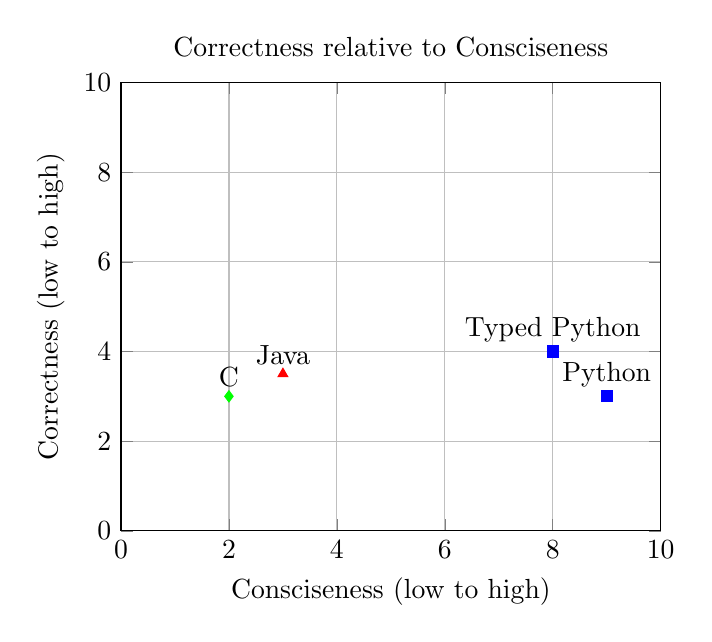
\begin{tikzpicture}
        \begin{axis}[
            xlabel={Consciseness (low to high)},
            ylabel={Correctness (low to high)},
            xmin=0, xmax=10,
            ymin=0, ymax=10,
            grid=major,
            legend pos=north west,
            title={Correctness relative to Consciseness}
        ]
        % Points for each language
        \addplot[only marks, mark=square*, color=blue] coordinates {(9, 3)}; % Python
        \addplot[only marks, mark=square*, color=blue] coordinates {(8, 4)}; % typed Python
        \addplot[only marks, mark=triangle*, color=red] coordinates {(3, 3.5)}; % Java
        \addplot[only marks, mark=diamond*, color=green] coordinates {(2, 3)}; % C
        % \addplot[only marks, mark=star, color=purple] coordinates {(1, 1)}; % asm
    
        % Adding labels for languages
        \node at (axis cs:9,3) [anchor=south] {Python};
        \node at (axis cs:8,4) [anchor=south] {Typed Python};
        \node at (axis cs:3,3.5) [anchor=south] {Java};
        \node at (axis cs:2,3) [anchor=south] {C};
        % \node at (axis cs:1,1) [anchor=south] {asm};
        \end{axis}
    \end{tikzpicture}
    \caption{A comparison of programming languages on consciseness and correctness.}
    \label{fig:language_comparison}
\end{figure}

\comment{Because of the fact that I don't have data to place the "Typed Python" on the figure properly, this feels a lot less informative and scientific than I originally thought. Maybe cut.}

Demonstrative figure \ref{fig:language_comparison} describes Python and Typed Python relative correctness and consciseness properties compared to other programming languages. Correctness refers to how many constructs and validations the language provides to ensure that programs are correct. Consciseness refers to the amount of required source code to achieve a certain function.

The figure is based on a study of various programming languages performance on Rosetta Code tasks \cite{nanz_comparative_2015}. They do not generalize to generic programs, but they are indicative and the relations are consistent with other research \cite{ray_codequality_2014}. (All the Python code in the study was untyped, since Python type annotations were not adopted before 2015. Typed Python was not researched in the study, and is a hypothetical addition.)

Python has apparently managed to arrive at a useful compromise on readability, expressivity and syntactic noise. Gradual typing provides a way to increase readability and correctness, with a cost of additional syntactic noise.

\subsection{Gradually typing Python}
Benefits of gradual typing: Gradual types work as documentation for internal and external APIs. Gradual types can be utilized to focus correctness efforts in the code base to the spots where they make most sense \cite{di_grazia_evolution_2022}.

\comment{TODO: expand on benefits / features of gradual typing}

\comment{\subsection{Why type check Python} TODO: type checking Python is easier than ever due to tooling improvements (Take some text from part 2.3.1 to here)}
\chapter{Conclusions\label{conclusions}}

Python is adopted for a wide variety of reasons, including ease of use, ease of learning, and the wide availability of packages. In comparison to other programming languages it lands at an useful compromise on readability, expressivity and syntactic noise.

Type annotations are being adopted more widely due to maintenance benefits and easing the detection of bugs \cite{jin_where_to_start_2021, khan_empirical_2022}. Utilizing gradual types makes Python into a gradually typed programming language, with increased readability, self-documentation and correctness, with costs in additional syntactic noise and additional development effort.  

Type checking has been made easier by popularity of editors that do it by default. This helps developers find bugs and utilize type information. Type-annotated Python allows developers to utilize Pythons core strengths while improving on shortcomings that have historically widely applied to dynamic scripting languages.

Projects should adopt Python type annotations when they want to spend development efforts on improving the maintainability, correctness, and static analysis of their code base. Intentions on coverage, specifically which internal and public APIs should end up covered, should be set. Some time should be spent on estimating where correctness and analysis improvements provide most benefit. Often this would be places where type annotation is not exceptionally difficult, and which often result in bugs. When type annotating proves difficult it can sometimes be a hint that program structure is complicated, and could benefit from refactoring.
% \cite{jin_where_to_start_2021}

There are avenues for future research on utilizing Python type annotation most effectively, comparing type checkers, and figuring out what the adoption rate and quality of type hints has been since 2022. Research to use the type annotations for performance and correctness benefits in runtime, and popularity of existing solutions could be useful. There is also demand for explanations on how to adopt type hints.

% Considering size of Python there seem to be lots of untapped avenues for future research.

%%%%%%%%%%%%%%%%%%%%%%%%%%%%%%%%%%%%%%%%%%%%%%%%%%%%%%%%%
%\cleardoublepage                          %fixes the position of bibliography in bookmarks
%\phantomsection
\addcontentsline{toc}{chapter}{\bibname}  % This lines adds the bibliography to the ToC
\printbibliography

%%%%%%%%%%%%%%%%%%%%%%%%%%%%%%%%%%%%%%%%%%%%%%%%%%%%%%%%%
\backmatter
\begin{appendices}

%% A sample Appendix

\appendix{Use of AI \label{appendix:ai}}

ChatGPT 4-o was used to generate LaTeX source code for figures \ref{untyped_code}, \ref{typed_code}, \ref{fig:language_comparison} and table \ref{table:1}. 

Claude 3.5 Haiku was used to spell check the Lyhennelmä in Finnish.

Overleafs Writefull integration was used for spell checking.
%% another appendix
% \include{instructions/instructions_english}
%% yet another appendix
% \include{instructions/instructions_finnish}

% BSc instructions
%\include{instructions/bsc_finnish_contents}
%\include{instructions/bsc_english_contents}


\end{appendices}
%%%%%%%%%%%%%%%%%%%%%%%%%%%%%%%%%%%%%%%%%%%%%%%%%%%%%%%%%

\end{document}
